
\begin{center}
\Huge
	Mere om faktorisering
\end{center}
\section*{Bestemmelse af rødder ved faktorisering}
\stepcounter{section}

Vi betragter fortsat andengradspolynomier $p$ på formen
\begin{align*}
	p(x) = ax^2 + bx + c,
\end{align*}
men i dette tilfælde holder vi os til tilfældet, at $a = 1$. Vi skal se, hvordan vi kan bestemme rødderne for et andengradspolynomium ved at faktorisere det. Lad derfor $x_1$ og $x_2$ være rødder for $p$. Vi faktoriserer så $p$ og hæver parenteserne.
\begin{align*}
	p(x) &= (x-x_1)(x-x_2)\\
	&= x^2 -xx_1 - xx_2 + (-x_1)(-x_2)\\
	&= x^2 \underbrace{- (x_1+x_2)}_{=b}x + \underbrace{x_1x_2}_{=c}.
\end{align*}
Ud fra dette må der gælde, at 
\begin{align*}
	b = -(x_1 + x_2),
\end{align*}
og
\begin{align*}
	c = x_1x_2.
\end{align*}
Vi kan altså ved at finde to tal der ganget sammen giver $c$ og lagt sammen giver $-b$ finde rødderne for $p$. Betragt følgende eksempel.
\begin{exa}
	Lad et andengradspolynomium $p$ være givet ved
	\begin{align*}
		p(x) = x^2 - 6x + 8.
	\end{align*}
	Vi ved, at $b = -6$ og $c = 8$. Vi skal altså finde to tal $x_1$ og $x_2$, så
	\begin{align*}
		8 = x_1x_2
	\end{align*}
	og
	\begin{align}\label{eq:b}
		-6 = -(x_1 + x_2)\ \Leftrightarrow \ 6 = x_1 + x_2.
	\end{align}
	Det er typisk nemmest at opskrive $c = 8$ i primtalsfaktorer. Da $8 = 2\cdot 2 \cdot 2$, så er den ene rod 
	$\pm 2$, $\pm 4$ eller $\pm 8$.
	Vi prøver med 4, og sætter dette ind i \eqref{eq:b}. Dette giver
	\begin{align*}
		6 = 4 + x_2
	\end{align*}
	og vi får herfra at $x_2 = 2$. Vi har derfor fundet rødderne $x_1 = 4$ og $x_2 = 2$.  
\end{exa}

\section*{Toppunkter for parabler}
\stepcounter{section}

Vi kalder det sted, hvor en parabel har ekstremum for et \textit{toppunkt} ligegyldigt om det er et maksimum eller minimum. På Figur \ref{fig:toppunkt} kan toppunkterne for to parabler ses.
\begin{figure}[H]
	\centering
	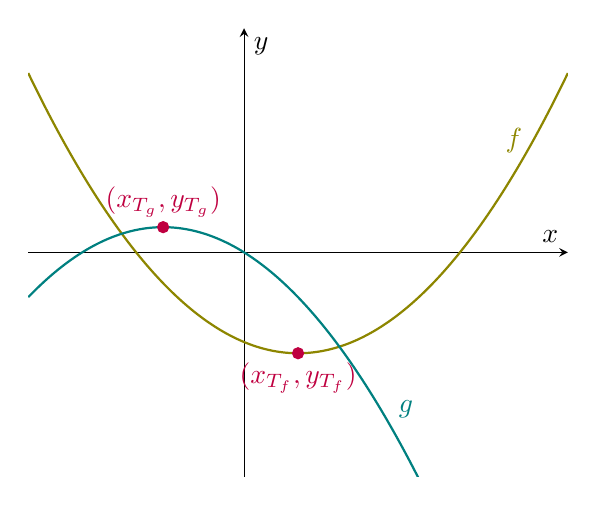
\begin{tikzpicture}
		\begin{axis}[
		axis lines = center, 
		xmin = -4, xmax = 6,
		ymin = -20, ymax = 20,
		ticks = none, 
		xlabel = $x$, ylabel = $y$
		]
			\addplot[color = olive, thick, domain = -4:6, samples = 300] {(x+2)*(x-4)};
			\addplot[color = teal, thick, domain = -4:6, samples = 300] {-(x+3)*(x)};
			\filldraw[color = purple] (axis cs: 1,-9) circle (2pt);
			\filldraw[color = purple] (axis cs: -3/2,9/4) circle (2pt);
			\node[color = purple, anchor = north] at (axis cs: 1,-9) {$(x_{T_f},y_{T_f})$};
			\node[color = purple, anchor = south] at (axis cs: -3/2,9/4) {$(x_{T_g},y_{T_g})$};
			\node[color = olive] at (axis cs: 5,10) {$f$};
			\node[color = teal] at (axis cs: 3,-14) {$g$};
		\end{axis}
	\end{tikzpicture}
	\caption{Toppunkter for to parabler for andengradspolynomierne $f$ og $g$.}
	\label{fig:toppunkt}
\end{figure}
Vi har følgende sætning, der beskriver, hvordan man kan finde toppunkter for andengradspolynomier. 
\begin{setn}[Toppunkter for parabler]
	Lad et andengradspolynomium $p$ være givet ved
	\begin{align*}
		p(x) = ax^2 + bx + c.
	\end{align*}
	Så kan koordinatsættet til toppunktet for $p$ findes ved
	\begin{align*}
		\left(x_T,y_T\right) = \left(\frac{-b}{2a}, \frac{-d}{4a} \right).
	\end{align*}
\end{setn}
Vi vil først bevise sætningen senere, når vi har værktøjet \textit{differentialregning} til rådighed. I stedet vil vi betragte et eksempel.
\begin{exa}
	Vi lader andengradspolynomiet $p$ være givet ved
	\begin{align*}
		p(x) = x^2 - 10x + 5,
	\end{align*}
	og vi ønsker at finde toppunktet. Vi finder først $x_T$.
	\begin{align*}
		x_T = \frac{-b}{2a} = \frac{10}{2} = 5.
	\end{align*}
	Vi finder så $y_T$.
	\begin{align*}
		y_T = \frac{-d}{4a} = \frac{-(10^2 - 4\cdot 1 \cdot 5)}{4} = \frac{-80}{4} = -20.
	\end{align*}
	Vi kan også indsætte førstekoordinaten $x_T = 5$ i funktionsudtrykket. Så får vi
	\begin{align*}
		p(5) = 5^2 - 10\cdot 5 + 5 = 25-50+5 = -20.
	\end{align*}
	På begge måder får vi koordinatsættet til toppunktet til at være 
	\begin{align*}
		\left(x_T,y_T\right) = \left(5,-20\right).
	\end{align*}
\end{exa}
\subsection*{Opgave 1}

Bestem rødderne for følgende andengradspolynomier ved at faktorisere dem. 
\begin{align*}
	&1) \ p(x) = x^2 + 2x - 15 &  &2) \ p(x) = x^2-4x + 3 \\
	&3) \ p(x) = x^2 - 2x - 8 &  &4) \ p(x) = x^2 + 6x + 9 \\
	&5) \ p(x) = x^2 + 11x + 30 &  &6) \ p(x) = x^2 + 3x - 10 \\
\end{align*}

\subsection*{Opgave 2}
Et andengradspolynomium $p$ har roden $x_1 = 2$, $a= 4$ og parablen for $p$ går gennem punktet $(3,4)$. 
\begin{enumerate}[label=\roman*)]
	\item Bestem værdien for den anden rod $x_2$. 
	\item Find $b$- og $c$-værdien for $p$. 
\end{enumerate}

\subsection*{Opgave 3}
Et andengradspolynomium $p$ er givet ved
\begin{align*}
	p(x) = x^2 + bx +c 
\end{align*}
og opfylder, at $p(0) = 5$ og $p(2) = 5$.
\begin{enumerate}[label=\roman*)]
	\item Bestem tallene $b$ og $c$. 
\end{enumerate}

\subsection*{Opgave 4}
Bestem koordinatsættet til toppunktet for følgende andengradspolynomier.
\begin{align*}
	&1) \ p(x) = x^2 &  &2) \ p(x) = \frac{1}{2}x^2 + 1x + 1 \\
	&3) \ p(x) = 2x^2 - 4x + 2 &  &4) \ p(x) = -x^2 + 6x - 4 \\
	&5) \ p(x) = -3x^2 + 9x + 5 &  &6) \ p(x) = 5x^2 -2x + 6 \\
\end{align*}

\subsection*{Opgave 5}
Et andengradspolynomium $p$ har $a = 1$ og rødderne $x_1 = 5$ og $x_2 = -2$.
\begin{enumerate}[label=\roman*)]
	\item Bestem koordinatsættet til toppunktet for $p$.
\end{enumerate}  

\subsection*{Opgave 6}
På Figur \ref{fig:toppunktopgave} ses parablen for et andengradspolynomium $p$. 
\begin{figure}[H]
	\centering
	\begin{tikzpicture}
		\begin{axis}[
		axis lines = center, 
		xmin = -4, xmax = 6,
		ymin = -20, ymax = 20,
		ytick = {8},
		xtick = {-3,1,2},
		xlabel = $x$, ylabel = $y$
		]
			\addplot[color = olive, thick, domain = -4:6, samples = 200] {-2*(x-2)*(x+3)};
			\filldraw[color = teal] (axis cs: 1,8) circle (2pt);
			\draw[color = teal, dashed, thick] (axis cs: 1,0) -- (axis cs: 1,8);
			\draw[color = teal, dashed, thick] (axis cs: 0,8) -- (axis cs: 1,8);
		\end{axis}
	\end{tikzpicture}
	\caption{Parabel for andengradspolynomiet $p$.}
	\label{fig:toppunktopgave}
\end{figure}
\begin{enumerate}[label=\roman*)]
	\item Bestem $a$-værdien for $p$. 
	\item Opskriv faktoriseringen for $p$. 
	\item Bestem toppunktet for $p$. 
\end{enumerate}

\subsection*{Opgave 7}
Vi vil gerne bevise faktoriseringssætningen fra sidst. 
\begin{enumerate}[label=\roman*)]
	\item Hæv parentesen i udtrykket $a(x-x_1)(x-x_2)$
	\item Betragt udtrykket. Hvad tilsvarer $b$ og hvad tilsvarer $c$?
	\item Indsæt udtrykket for rødderne fra diskriminantformlen i udtrykkene for $b$ og $c$ og vis, at 
	udtrykket bliver sandt. 
	\item Sæt en sort firkant.